%%%%%%%%%%%%%%%%%%%%%%%%%%%%%%%%%%%%%%%%%%%%%%%%%%%%%%%%%%%%%%%%%%%%%%%
\documentclass
  [ 12pt
  %twoside            % beidseitiger Druck
  , openright          % Kapitel beginnen auf einer rechten Seite
  , listof=totoc       % Verzeichnisse im Inhaltsverzeichnis
  , bibliography=totoc % Literaturverzeichnis im Inhaltsverzeichnis
  , parskip=full       % Absätze durch einen vergrößerten Zeilenabstand getrennt
%  , draft              % Entwurfsversion
  ]{scrreprt}          % Dokumentenklasse: KOMA-Script Buch

\input{stuff/header}

\begin{document}

%%%%%%%%%%%%%%%%%%%%%%%%%%%%%%%%%%%%%%%%%%%%%%%%%%%%%%%%%%%%%%%%%%%

% Titelseite
\newgeometry{left=3cm,right=2cm,top=2.0cm,bottom=2.0cm}
\include{stuff/titelseite}
\restoregeometry

%%%%%%%%%%%%%%%%%%%%%%%%%%%%%%%%%%%%%%%%%%%%%%%%%%%%%%%%%%%%%%%%%%%

% Mehr Platz für Nummerierung benötigt in Verzeichnissen, wenn ein Kapitel 10 oder mehr Bilder hat
\DeclareTOCStyleEntry[numwidth=3em]{tocline}{figure} % Für Abbildungsverzeichnis
%\DeclareTOCStyleEntry[numwidth=3em]{tocline}{table} % Für Tabellenverzeichnis

\pagenumbering{Roman}

\tableofcontents
\listoffigures
\listoftables
\cleardoublepage

%%%%%%%%%%%%%%%%%%%%%%%%%%%%%%%%%%%%%%%%%%%%%%%%%%%%%%%%%%%%%%%%%%%

\pagenumbering{arabic}

\begin{onehalfspace}
\chapter{Einleitung}
\label{chap: intro}

Hier kommt die Einleitung hin ...

\chapter{Architektur}
\newpage

\section{Data-Ingestion Pipeline}

\begin{figure}[h!]
    \centering
    \includegraphics[scale=1.5]{bilder/architektur-data-ingestion.pdf}
    \caption[Überblick Data Ingestion Pipeline]{Überblick Data Ingestion Pipeline}
    \label{fig:data ingestion arch}
\end{figure}

\newpage

\section{RAG-Pipeline}

\begin{figure}[h!]
    \centering
    \includegraphics[scale=0.74]{bilder/architektur-rag-pipeline.pdf}
    \caption[Überblick RAG Pipeline]{Überblick RAG Pipeline}
    \label{fig:rag pipe arch}
\end{figure}

\newpage

\section{Query Processing Pipeline}

\begin{figure}[h!]
    \centering
    \includegraphics[scale=0.74]{bilder/architektur-query-processing-pipeline.pdf}
    \caption[Query Processing Pipeline]{Query Processing Pipeline}
    \label{fig:query processing arch}
\end{figure}
\include{kapitel/Preprocessing}
\chapter{Chunking und Embedding Strategien}
\label{chap:chunking}

\section{Überblick}

Die Architektur der Pipeline gliedert sich in die Teile Indexierung, Retrieval und Generation, welche in den folgenden Abschnitten näher erklärt werden. Die Indexierung beinhaltet die Erstellung der Markdown-Dateien durch verschiedene Parser, sowie die Erstellung und das Embedding strukturierter Chunks mit anschließender Speicherung in der Vektordatenbank. Das Retrieval nutzt die Query, um durch Query Expansion, hybride Suchansätze und Reranking die relevantesten Inhalte an das LLM für die Generierung zu liefern. Bei der Generierung werden außerdem verschiedene Prompt-Templates für eine verbesserte Antwort genutzt.

Die verwendeten Technologien sind in der  folgenden Tabelle zu sehen.
\begin{table}[htbp]
\centering
\begin{tabular}{|l|p{8.5cm}|}
\hline
\textbf{Komponente} & \textbf{Technologie} \\
\hline
Framework & Haystack 2.x \\
Vektordatenbank & Qdrant (lokal) \\
Embedding-Modell & OpenAI text-embedding-3-small (1536 Dimensionen) \\
LLM & OpenAI gpt-4o-mini \\
Dokumentformat & Markdown (konvertiert aus PDFs) \\
\hline
\end{tabular}

\caption{Verwendete Komponenten und Technologien}
\label{tab:komponenten_technologien}

\end{table}
\section{Chunking-Strategien}

\subsection{Parsing}
Das Grundprinzip des Chunkings ist das Dokumenttypspezifische Parsing, da generisches Chunking für die strukturierten Dokumente ungeeignet war. Hierbei werden die verschiedenen Dokumente, je nach Typ, anders gechunkt und mit Metadaten angereichert. Die wichtigsten Parser sind hierbei die folgenden drei Hauptparser und ein Base-Parser für normalen unstrukturierten Text. Im folgenden Code ist die Auswahl der Parser zu sehen, die je nach Dokumenttyp ausgewählt werden.

\begin{lstlisting}[language=Python, caption={Parser Auswahl}]
PARSERS = [
    CurriculumParser(),  # Studienverlaufsplaene
    ModulhandbuchParser(),   # Modulhandbuecher  
    RegulationsParser(),  # SPO, PVO, ZLO
]

def select_parser(filename: str):
    if "CURRICULUM" in filename.upper():
        return CurriculumParser()
    if "MODULHANDBUCH" in filename.upper():
        return ModulhandbuchParser()
    if re.match(".*(SPO|PVO|ZLO|RICHTLINIEN).*", filename.upper()):
        return RegulationsParser()
    return None  # Fallback
\end{lstlisting}

\subsubsection{Curriculum-Parser}
Der Curriculum-Parser befasst sich mit allen Studienverlaufsplänen und Curricula. Der Schwerpunkt liegt hier darin die einzelnen Module mit allen Daten wie Semesterzuordnungen und ECTS aus den Markdown Tabellen zu extrahieren. Die Tabellen haben in Markdown die folgende Form:

| MB001 Analysis<br>TB001<br>... | ... | 5 | | | | | | | |

Der Parser wurde implementiert, so dass er die verschiedenen Informationen aus den Spalten extrahiert und einzeln speichert. Hierfür wird das Dokument zuerst in Zeilen unterteilt und dann werden die einzelnen Spalten analysiert. Anschließend wird die vollständige Modulliste durch die Kombination der einzelnen Werte gebaut.
\begin{lstlisting}[language=Python, caption={Regulatinsparser-Implementierung}]
def parse(self, path: Path, meta: Dict) -> List[Document]:

    # Sammle Semester- und ECTS-Informationen
    for line in lines:
        cells = self._parse_table_row(line)
        code = self._extract_module_code(cells)
        semester = self._detect_semester(cells)  # Aus ECTS-Spalten
        ects = self._extract_ects(cells)         # Summe der Spalten
        module_semesters[code] = semester
        module_ects[code] = ects
    
    # Baue vollstaendige Modulliste
    for line in lines:
        code, title = self._extract_module_info(cell)
        modules.append({
            "code": code,
            "title": title,
            "semester": module_semesters.get(code),
            "ects": module_ects.get(code),
        })
\end{lstlisting}

Die erzeugten Chunks gliedern sich in die drei Typen Modulübersicht, Semesterübersicht und Moduldetail, die in der folgenden Tabelle ersichtlich sind. 

\begin{table}[htbp]
\centering
\begin{tabular}{|p{3.6cm}|p{4.8cm}|p{8.0cm}|}
\hline
\textbf{Chunk-Typ} & \textbf{Beschreibung} & \textbf{Beispielinhalt} \\
\hline
module\_overview & Gesamtuebersicht aller Module & Modulübersicht für Informatik (Bachelor) \dots Anzahl Module: 42 \\
semester\_overview & Module pro Semester & Module im 3. Semester -- Informatik (Bachelor) \dots Gesamt-ECTS: 30 \\
module\_detail & Einzelnes Modul mit Kontext & Modul MB001: Analysis, Semester 1, ECTS: 5 \\
\hline
\end{tabular}
\caption{Verwendete Chunk-Typen}
\label{tab:chunk_typen}
\end{table}

Die Herausforderungen und Lösungen beim Parsing von Curriculum-Dateien sind hier dargestellt:

\begin{table}[htbp]
\centering
\begin{tabular}{|p{8.0cm}|p{8.0cm}|}
\hline
\textbf{Problem} & \textbf{Lösung} \\
\hline
Modulnamen über \texttt{<br>}-Tags verteilt & Regex-basierte Extraktion mit Fallback auf Folgezeilen \\
ECTS verteilt über 7 Semesterspalten & Summierung aller positiven Werte in den Spalten 3--9 \\
Fehlende Semesterzuordnung & Erkennung anhand der Spalte mit positivem ECTS-Wert \\
\hline
\end{tabular}
\caption{Probleme und Loesungen bei der Extraktion}
\label{tab:probleme_loesungen}
\end{table}

\subsubsection{Modulhandbuch-Parser}
Der Modulhandbuch Parser extrahiert strukturierte Modulbeschreibungen mit Lernzielen und Inhalten aus den Modulhandbüchern. Die verschiedenen Sektionen werden hier  über ihre Bezeichner erkannt.

\begin{lstlisting}[language=Python, caption={Sektionen}]
SECTION_HEADERS = [
    "Modulname", "Modultitel", "Modulnummer", "Studiengang", "Semester",
    "Voraussetzungen", "Lernziele", "Inhalte", "Arbeitsaufwand",
    "Pruefungsform", "Literatur", "Dozent", "Lehrform"
]
\end{lstlisting}

Die Chunking-Strategie reduziert die maximale Chunkgröße auf 450 Zeichen, was für die Embeddings optimal ist und jeder Chunk erhält einen Kontext-Header mit folgender Struktur:

\begin{lstlisting}[language=Python, caption={Kontext-Header}]
context_header = f"Modul: {module_name}\nStudiengang: {program} ({degree})\n\n"
chunk_content = context_header + f"Abschnitt: {subsection}\n" + content
\end{lstlisting}

Die erzeugten Dokumente sind die Modulübersicht, welche eine Liste aller Module im Handbuch enthält und die Sektions-Chunks, die die einzelnen Abschnitte pro Modul wie Lernziele beinhalten. So können die verschiedenen Informationen den konkreten Modulen direkt zugewiesen werden, was im Retrieval Prozess sehr nützlich ist.

\subsubsection{Regulations-Parser}
Der Regulations-Parser extrahiert einzelne Paragraphen aus den Prüfungs- und Studiengangsordnungen (SPO, PVO, ZLO). Das geschieht über ein Regex-Muster, welches die Paragraphen erkennt  und die jeweiligen Sektionen und Absätze unterteilt.
Die entstehenden Chunks bestehen aus den einzelnen Paragraphen mit einem Kontext-Header, um den Studiengang und Abschluss zu speichern. Die Chunkstruktur sieht wie folgt aus:

\begin{lstlisting}[language=Python, caption={Regulations Chunks}]
# Jeder Paragraph wird zu einem Chunk mit Kontext-Header
context_header = f"Pruefungsordnung {program} ({degree}) an der FH Wedel\n"
content = context_header + raw_paragraph_content
\end{lstlisting}

Die Metadaten jedes Chunks sind die Sektion wie z.B. "I. Allgemeines", der Paragraph mit der entsprechenden Nummer und der Paragraph-Titel wie z.B. "Regelstudienzeit". Diese Unterteilung auf einzelne Paragraphen mit den entsprechenden Metadaten erlaubt eine gute Einordnung und Speicherung der Texte für den nachfolgenden Retrieval-Prozess.

\subsection{Metadaten-Injektion}
Ein Konzept, das die Retrieval-Qualität verbessert ist außerdem die direkte Metadaten-injektion, so dass die Chunks die Metadaten direkt in ihren Content gespeichert bekommen, um die semantische Suche zu verbessern. Das geschieht, indem ein Kontext schrittweise mit allen verfügbaren Metadaten gefüllt wird und dann an den Anfang des Chunks gehängt wird. Der Ablauf ist hier zu sehen.
\begin{lstlisting}[language=Python, caption={Metadaten Injektion}]
def build_embed_text(doc: Document) -> str:
    context_parts = []
    
    if meta.get("degree"):
        context_parts.append(f"Studienabschluss: {meta['degree']}")
    if meta.get("program"):
        context_parts.append(f"Studiengang: {meta['program']}")
    if meta.get("doctype"):
        context_parts.append(f"Dokumenttyp: {meta['doctype']}")
    if meta.get("semester"):
        context_parts.append(f"Semester: {meta['semester']}")
    if meta.get("ects"):
        context_parts.append(f"ECTS: {meta['ects']}")
    # ...
    
    context_header = "Kontext: " + ", ".join(context_parts) + "."
    return f"{context_header}\n\n{doc.content}"
\end{lstlisting}

Dadurch entsteht ein Output in dieser Form, was die semantische Suche deutlich verbessert:

\subsection{Deduplizierung}
Um die Chunk-Anzahl zu reduzieren und einer Redundanz im Retrieval entgegen zu wirken, wurde außerdem eine Deduplizierung implementiert, die identische Chunks aus verschiedenen Versionen entfernt. Dadurch konnte die Chunk-Anzahl von 69000 auf 44500 Chunks gesenkt werden.

\section{Retrieval-Strategien}
Das zentrale Konzept des Retrieval-Prozesses ist das hybride Retrieval, also die Kombination aus Keyword-Suche und semantischer Suche für die optimale Abdeckung. Anschließend werden die Scores kombiniert und durch Query-Intention-Matching und Studiengangs-Matching angepasst. Diese Chunks werden anschließend durch verschiedene Reranking Algorithmen neu angeordnet, um eine maximale Relevanz zu gewährleisten.
\subsection{Hybrid Search}
Die hybride Suche unterteilt sich in die Keyword-Suche und die semantische Suche.
Bei der Keyword Suche werden die Vorkommen von Keywords im Chunk betrachtet, wobei besonders lange und aussagekräftige Wörter bevorzugt werden. Der Ablauf ist im folgenden zu sehen.

\begin{lstlisting}[language=Python, caption={Keyword Matching}]
def keyword_search(query: str, top_k: int, keywords: List[str]) -> List[Document]:
    # Alle Dokumente laden (fuer lokales Qdrant)
    all_docs = store.filter_documents()
    
    matched_docs = []
    for doc in all_docs:
        content_lower = doc.content.lower()
        # Score = Anteil der gefundenen Keywords
        matches = sum(1 for kw in keywords if kw in content_lower)
        if matches > 0:
            doc.score = matches / len(keywords)
            matched_docs.append(doc)
    
    return sorted(matched_docs, key=lambda d: d.score, reverse=True)[:top_k]
\end{lstlisting}

Bei der semantischen Suche wird die Nutzeranfrage zuerst in ihre Vektorrepräsentation umgewandelt und dann vom Retriever verwendet, um anhand semantischer Ähnlichkeit die relevantesten Chunks aus der Vektordatenbank abzurufen. Der Vorgang ist im folgenden Code-Abschnitt sichtbar.


\begin{lstlisting}[language=Python, caption={Semantische Suche}]
def semantic_search(query: str, top_k: int) -> List[Document]:
    embedder = OpenAITextEmbedder(model="text-embedding-3-small")
    retriever = QdrantEmbeddingRetriever(document_store=store)
    
    query_embedding = embedder.run(text=query)["embedding"]
    return retriever.run(query_embedding=query_embedding)["documents"]
\end{lstlisting}

\subsection{Score Fusion}
Nach der erfolgreichen hybriden Suche werden die Punkte kombiniert und eine Intentionserkennung durchgeführt, um anhand der Metadaten zu bestimmen, welche Dokumenttypen am relevantesten sind. Dies geschieht auf Basis von Modul und Regulations-Keyword Matching und ist im folgenden zu sehen.
Nach Bestimmung der Nutzerintention erhalten Chunks mit entsprechenden Dokumenttypen einen Punkte-Boost von 0,2 bis 0,25 Punkten.

\begin{lstlisting}[language=Python, caption={Semantische Suche}]
REGULATION_KEYWORDS = [
    "regelstudienzeit", "pruefung", "klausur", "zulassung", "voraussetzung",
    "pruefungsordnung", "frist", "thesis", "ects", "creditpoints", ...
]

MODULE_KEYWORDS = [
    "modul", "vorlesung", "lernziel", "inhalt", "dozent",
    "curriculum", "studienverlauf", "semester", ...
]

# Detect Intent
def detect_query_intent(query: str) -> str:
    regulation_score = sum(1 for kw in REGULATION_KEYWORDS if kw in query.lower())
    module_score = sum(1 for kw in MODULE_KEYWORDS if kw in query.lower())
    
    if regulation_score > module_score:
        return "regulation"
    elif module_score > regulation_score:
        return "module"
    return "general"

# Boosting
if query_intent == "regulation":
    if "spo" in filename or "pvo" in filename:
        doc_scores[doc_id] += 0.25    # Boost fuer SPO/PVO
elif query_intent == "module":
    if "modulhandbuch" in filename:
        doc_scores[doc_id] += 0.25    # Boost fuer Modulhandbuch
    elif "curriculum" in filename:
        doc_scores[doc_id] += 0.20
\end{lstlisting}

\subsection{Reranking}

Nach dem Retrieval werden die relevantesten Chunks nochmal durch verschiedene Reranking Methoden sortiert. Die erste Methode hierfür ist das Keyword basierte Reranking durch den BM25-Algorithmus. BM25 ist ein probabilistischer Ranking Algorithmus für Information Retrieval und bewertet wie relevant ein Dokument für eine Suchanfrage ist, basierend auf Term Frequency also wie oft ein Suchbegriff vorkommt, Document Length Normalization, so dass längere Dokumente keine unfairen Vorteile haben und Saturation, also dass häufigere Vorkommen abnehmenden Nutzen haben.

Die zweite Methode ist das LLM-basierte Reranking, wobei alle Chunks mit der Anfrage an ein LLM übergeben werden, welches diese neu sortiert und eine Reihenfolge nach Relevanz zurückgibt. Diese Methode ist optional und kann über ein Flag gesetzt werden, sorgt allerdings für bessere Resultate. Der Prompt für das Reranking Modell ist in folgendem Code zu sehen:

\begin{lstlisting}[language=Python, caption={Reranking Prompt}]
BATCH_RERANK_PROMPT = """Du bist ein Experte fuer Relevanz-Bewertung.

Frage: {query}

Hier sind {num_chunks} Textabschnitte. Sortiere sie nach Relevanz.
Gib NUR die Chunk-Nummern zurueck, sortiert vom relevantesten zum unwichtigsten.
Format: Eine Zeile mit kommagetrennten Nummern, z.B.: 3,1,5,2,4

{chunks}

Sortierte Reihenfolge (nur Nummern):"""
\end{lstlisting}

Eine weitere wichtige Funktionalität ist die Query Expansion, bei der die Nutzeranfrage durch ein LLM umgeschrieben wird, um das semantische Retrieval deutlich zu verbessern. Hierbei werden Synonyme, Keywords und andere relevante Wörter hinzugefügt und die Anfrage so umgeschrieben, dass der Kontext bzw. die Intention des Nutzers deutlicher ist und mögliche Rechtschreibfehler behoben. Der Prompt für die Query Expansion ist hier zu sehen:

\begin{lstlisting}[language=Python, caption={Query Expansion Prompt}]
def expand_query_with_llm(query: str, memory_summary: str, history) -> Tuple[str, str, List[str]]:
    prompt = f"""
    You rewrite user queries to improve semantic retrieval for a RAG system.
    
    Your tasks:
    1. Detect relevant context from the question
    2. Expand the query by adding synonyms, related keywords, module names
    3. You MUST NOT invent any new facts
    4. Always scope to "FH Wedel"
    
    User query: {query}
    
    Return JSON:
    {{
      "original_query": "<original>",
      "expanded_query": "<expanded retrieval query>",
      "keywords": ["keyword1", "keyword2", ...]
    }}
    """
    
    return expanded_query, original_query, keywords
\end{lstlisting}

\section{Generation}

 \subsection{Prompt Templates}
Der Hauptptompt für die meisten Anfragen ist der folgende:

\begin{lstlisting}[language=Python, caption={Generation Prompt}]
PROMPT_TEMPLATE = """
Du bist ein hilfreicher Assistent fuer die FH Wedel.
Beantworte die Frage **nur** basierend auf den bereitgestellten Dokumenten.
Wenn die Antwort nicht in den Dokumenten enthalten ist, sage 
"Das kann ich anhand der vorliegenden Dokumente nicht beantworten."
Antworte auf Deutsch, es sei denn die Frage ist auf Englisch gestellt.

### Bisheriger Kontext
{{ memory_summary or "Keiner" }}

### Dokumente
{% for doc in documents %}
[Dokument {{ loop.index }}] {{ doc.meta.get("doctype") }} | {{ doc.meta.get("program") }}
{{ doc.content[:2500] }}
{% endfor %}

### Frage
{{ query }}

### Antwort
"""
\end{lstlisting}

Sollte der Chatbot allerdings erkennen, dass eine Vergleichsfrage vom Nutzer gestellt wurde über die Kontextdetection wird stattdessen der folgende Prompt an das LLM übergeben:

\begin{lstlisting}[language=Python, caption={Comparison Prompt}]
COMPARISON_PROMPT_TEMPLATE = """
Du bist ein hilfreicher Assistent fuer die FH Wedel.
Der Nutzer moechte einen Vergleich zwischen zwei Dingen.

Strukturiere deine Antwort wie folgt:
1. Kurze Beschreibung von {{ entity1 }}
2. Kurze Beschreibung von {{ entity2 }}
3. Wichtige Unterschiede
4. Gemeinsamkeiten (falls relevant)

Basiere deine Antwort NUR auf den bereitgestellten Dokumenten.

### Dokumente
{% for doc in documents %}
[{{ doc.meta.get("comparison_entity") }}] {{ doc.meta.get("doctype") }}
{{ doc.content[:2000] }}
{% endfor %}

### Frage
{{ query }}
"""
\end{lstlisting}

\subsection{Generator Konfiguration}

Die Konfiguration des Chatbots lässt sich leicht anpassen, um andere Generationsmodelle oder deterministischere Antworten zu generieren. Die standard konfiguration sieht wie folgt aus:

\begin{lstlisting}[language=Python, caption={Comparison Prompt}]
generator = OpenAIGenerator(
    api_key=Secret.from_env_var("OPENAI_API_KEY"),
    model="gpt-4o-mini",
    generation_kwargs={
        "temperature": 0.3,    # Niedrig fuer faktische Antworten
        "max_tokens": 512,     # Standard-Antworten
    },
)
\end{lstlisting}

\section{Verworfene Ansätze}
Im Laufe der Entwicklung des Chatbots wurden viele Ansätze ausprobiert und wieder verworfen. Die wichtigsten Erkentnisse waren die folgenden:

1. Generisches Satzsplitting für alle Dokumente. Dieser Ansatz wurde schnell verworfen, da die wichtigen Informationen zertrennt wurden und vor allem Tabellen und andere strukturierte Daten viele Informationen und kontext verloren. Die Lösung hierfür war das Dokumentenspezifische Splitten über eigene Parser.

2. Reine semantische Suche. Da das Embeddingmodell relativ klein ist und die exakten Begriffe und deutsche Fachbegriffe oft nicht korrekt abgerufen wurden, wurde eine hybride Suche mit Keyword-Komponente integriert, was die Retrieval-Qualität stark verbesserte. 

3. Metadaten-Filter statt Injektion. Hier sollte die integrierte Qdrant Funktionalität zum Filtern von Begriffen verwendet werden, allerdings war diese zu restriktiv, so dass relevante Dokumente ausgeschlossen wurden.

4. Character-based Splitting. Das Splitten der Chunks in eine feste Zeichenanzahl von ca 500 Zeichen führte dazu, dass Sätze mitten im Wort abgeschnitten wurden und zusammenhängende Informationen und 
Kontext getrennt wurden, indem semantische Grenzen nicht respektiert wurden. Die Lösung hierfür war das Satz-basierte Splitting unstrukturierter Dokumente.

5. Während der Entwicklung kamen außerdem viele kleinere Probleme wie das korrekte Auslesen einzelner Paragraphen und ECTS oder die korrekte Speicherung der Metadaten, die alle schrittweise behoben wurden. Die Nutzung lokaler LLMs für die einzelnen API-Anfragen wurde auch verworfen, da die Antwortzeiten und Qualität der Antworten nicht ausreichend waren.

\section{Konfigurationsparameter}

Die Konfigurationsparameter, die der Nutzer anpassen kann, sind die folgenden:

\begin{table}[htbp]
\centering
\begin{tabular}{|l|l|l|p{5.8cm}|}
\hline
\textbf{Parameter} & \textbf{Wert} & \textbf{Datei} & \textbf{Beschreibung} \\
\hline
TOP\_K & 10 & config.py & Anzahl der finalen Chunks \\
MAX\_CHUNK\_SIZE & 450 & modulhandbuch\_parser.py & Maximale Chunk-Größe \\
split\_length & 5 & indexing\_pipeline.py & Sätze pro Chunk \\
split\_overlap & 1 & indexing\_pipeline.py & Überlappung in Sätzen \\
USE\_LLM\_RERANK & False & config.py & LLM-Reranking aktivieren \\
EMBEDDING\_DIM & 1536 & config.py & Embedding-Dimensionen \\
\hline
\end{tabular}
\caption{Wichtige Konfigurationsparameter}
\label{tab:konfigurationsparameter}
\end{table}

\section{Dateiübersicht}

Die relevantesten Dateien sind für besseres Verständnis hier aufgezeigt:

\begin{table}[htbp]
\centering
\begin{tabular}{|p{5.2cm}|p{8.2cm}|}
\hline
\textbf{Datei} & \textbf{Zweck} \\
\hline
indexing\_pipeline.py & Hauptpipeline für die Indexierung \\
hybrid\_retrieval.py & Implementierung der hybriden Suche \\
reranker.py & BM25 + LLM-Reranking \\
query\_expansion.py & Query-Erweiterung mit LLM \\
context\_detection.py & Kontext-Erkennung \\
rag\_pipeline.py & Generierung mit Prompts \\
curriculum\_parser.py & Parser für den Studienverlaufsplan \\
modulhandbuch\_parser.py & Parser für das Modulhandbuch \\
regulations\_parser.py & Parser fuer SPO/PVO/ZLO \\
document\_store.py & Qdrant-Konfiguration \\
\hline
\end{tabular}
\caption{Dateien und ihre Aufgaben}
\label{tab:dateien_zweck}
\end{table}








\chapter{Testing mit \emph{DeepEval}}
\label{chap:testing}

\section{Framework/Deepeval}

Die Wahl des Frameworks fiel auf Deepeval, da Deepeval die genaue Überprüfung der gesamten RAG-Pipeline in verschiedensten Systemen ermöglicht. DeepEval ist ein opensource  Python Framework speziell dafür entwickelt LLM Applikationen zu evaluieren. Hierfür können verschiedenste LLMs als Judge-Modelle genutzt werden, die basierend auf vorher definierten Metriken die Qualität der Antworten und Chunks bewerten. Außerdem ermöglicht Deepeval die native Integration durch Pytest, sowie multi-modale Evaluation und die automatische Optimierung von Prompts. Im Kontext des Chatbots bot sich die End-To-End LLM Evaluation von DeepEval an, da es sich um eine relativ simple Architektur handelt und die Anfragen nur Fragen und Anworten sind, die durch einen einzigen LLM-Testcase repräsentiert bzw. getestet werden können.

Hierbei wird eine einzelne Testinstanz über einen LLMTestCase abgebildet, welcher die Eingabe-Query, Ausgabe und den Retrieval-Kontext beinhaltet. Als Judge Modell stehen in dem Projekt zwei Implementationen bereit. Hierbei kann der Nutzer zwischen OpenAI und AWS Bedrock unterscheiden und die entsprechenden Modelle selbst auswählen. In den meisten Tests wurde das OpenAI Modell GPT-4o-mini genutzt. Es kann außerdem zwischen verschiedenen Metriken ausgewählt werden, welche daraufhin in jedem einzelnen Testfall geprüft werden und anhand eines  vorher definierten Threshhold Wertes von 0.0-1-0 kann definiert werden, ob ein Test fehlschägt oder erfolgreich ist.

\section{Überblick}
Der Aufbau ist in Abbildung \ref{fig:e2e} zu sehen.
\begin{figure}[h] 
    \centering
    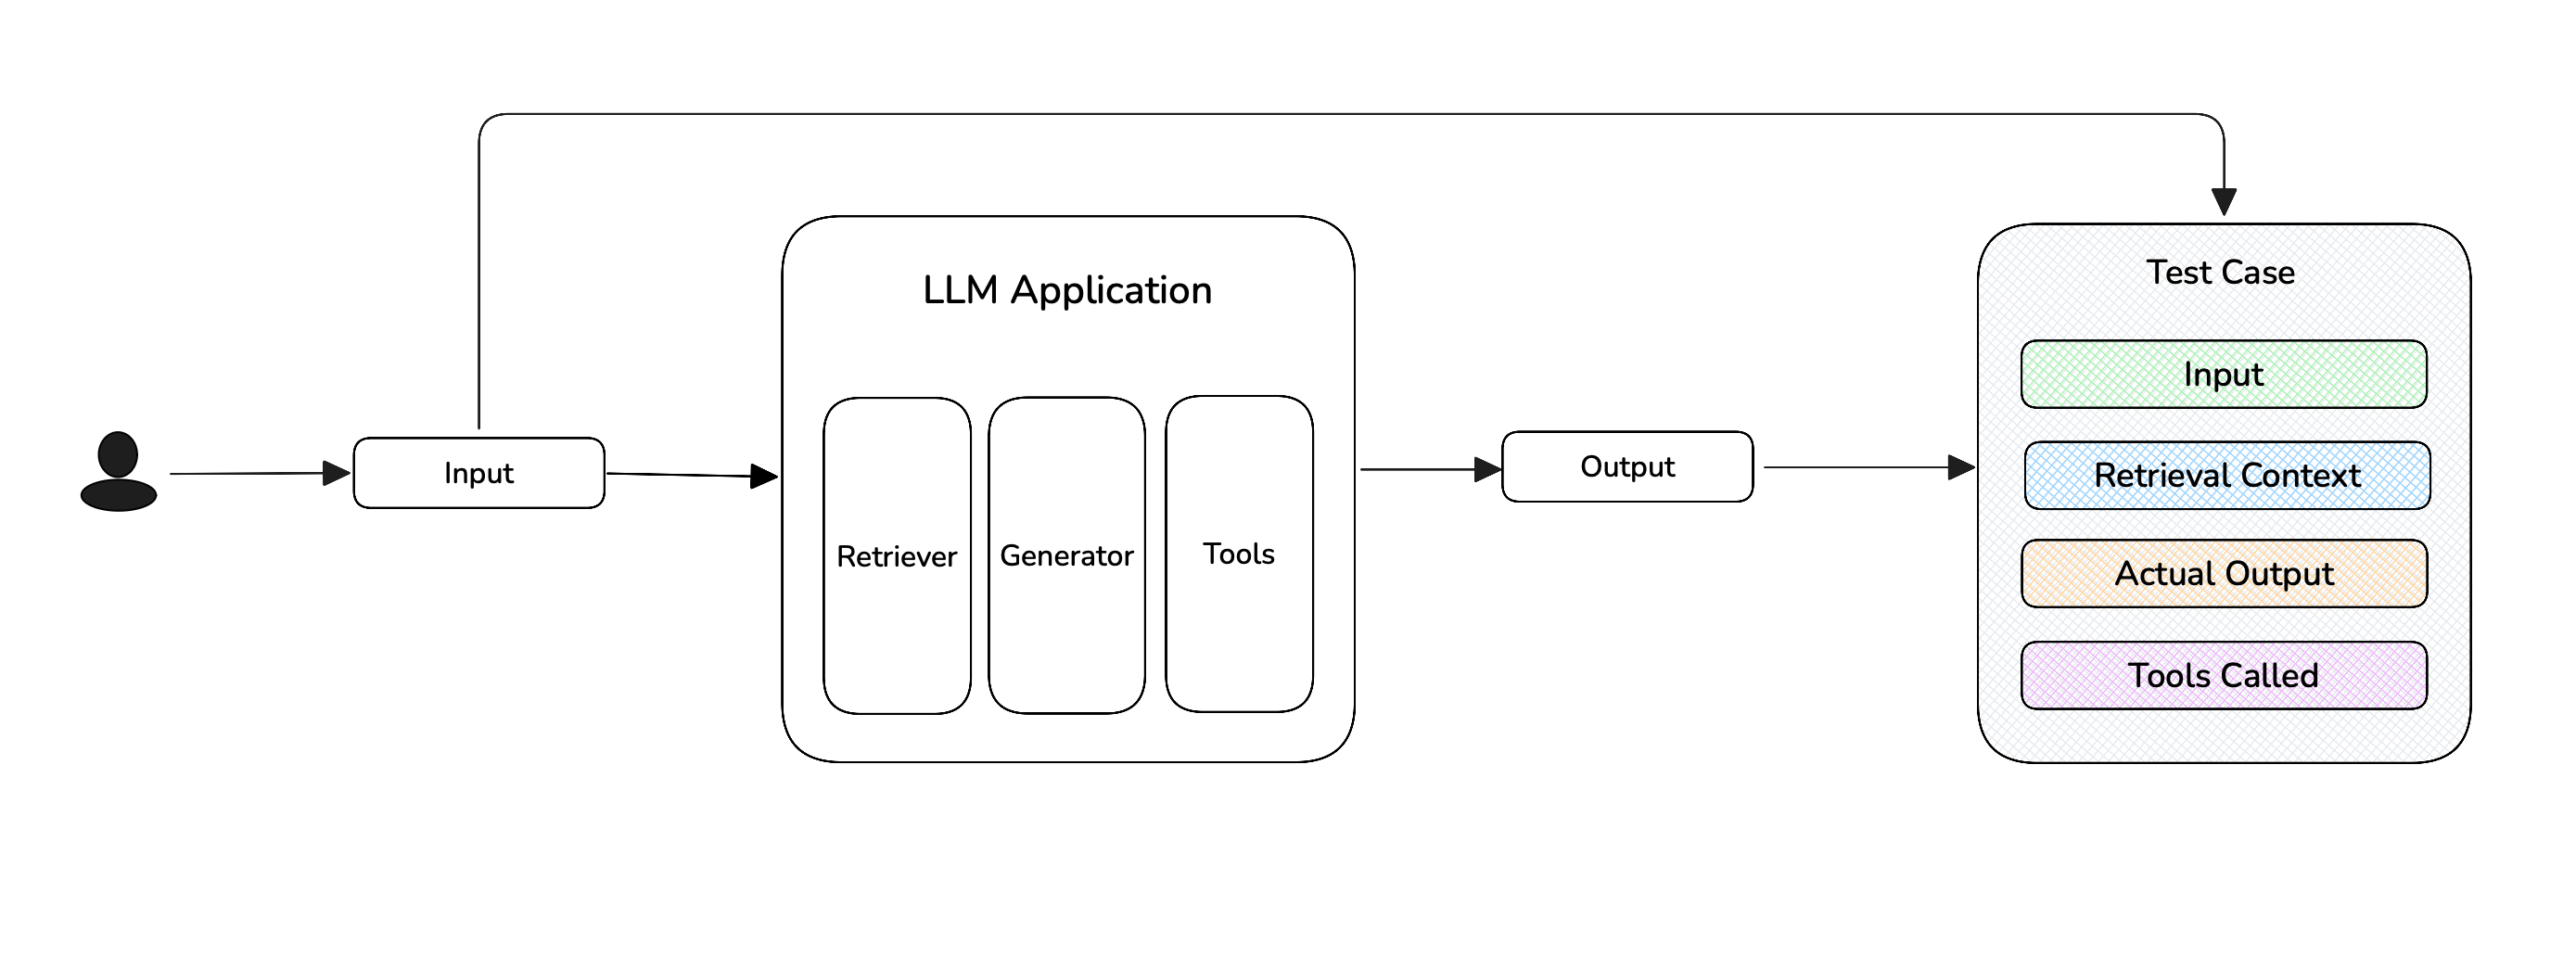
\includegraphics[width=0.8\textwidth]{bilder/e2e}\\
    \caption{End-To-End Evaluation}
    \label{fig:e2e}
\end{figure}

Hierbei wird die RAG-Pipeline als Blackbox behandelt und es werden nur die Eingaben und Ausgaben, sowie die benutzten Tools evaluiert.

Um einen Testdurchlauf zu starten kann der Nutzer einfach den Test Runner ausführen, welcher die gesamte RAG-Pipeline für jede der vordefinierten Queries durchläuft. Hierbei werden die retrieved Chunks und die Antwort gespeichert und anhand der Metriken bewertet.


\section{Metriken}
Wir haben uns in dem Projekt für die drei Metriken AnswerRelevancy, Faithfulness und ContextualRelevancy entschieden, um die wichtigsten Bereiche abzudecken und zu überprüfen.

\subsubsection{AnswerRelevancy}
Hierbei geht es darum zu identifizieren, ob die generierte Antwort relevant für die gestellte Frage ist. Es wird evaluiert, ob die Antwort tatsächlich das gefragte addressiert oder nicht und bewertet Antworten schlechter, die nicht zum Thema passen oder zu ungenau sind. Hierbei wird jedoch nicht geprüft, ob die Antworten faktisch korrekt sind. Der Threshhold ist hierbei 0.5 und eine beispielhafte, fehlerhatfe Anwort könnte so aussehen:

Query: \enquote{Wie viel ECTS hat Digitaltechnik?}\newline
Answer: \enquote{Die FH Wedel bietet viele Module an...} → Fails (doesn't answer question)

\subsubsection{Faithfulness}
Diese Metrik bezieht sich auf die generierten Chunks aus dem Retrieval Kontext. Hierbei wird überprüft, ob die generierte Antwort und jede einzelne Aussage auf den Chunks basiert. Das ist vorallem wichtig für die Halluzinationserkennung und essenziell für die Vertrauenswürdigkeit des Chatbots. Der Threshhold ist hierbei 0.5 und eine beispielhafte, fehlerhatfe Anwort könnte so aussehen:

Retrieved chunks mention \enquote{7 Semester Regelstudienzeit}\newline
Answer says \enquote{6 Semester} → Fails (hallucination)

\subsubsection{ContectRelevancy}
Diese Metrik bewertet die Relevanz und Qualität der Chunks bezüglich der Frage. Hierbei wird also der Retrieval-Prozess evaluiert und nicht die generierte Antwort. Der Threshhold ist hierbei nur  0.25, weil chunks oft extra Kontext beinhalten und eine beispielhafte, fehlerhatfe Anwort könnte so aussehen:

Query: \enquote{Prüfungsordnung Bachelor Informatik}\newline
Retrieved chunks: Curriculum tables, module descriptions → Fails (wrong doc types)

\section{Judge Models}
Anfangs wurde der Ansatz lokale Modelle für die Evaluierung zu nutzen verfolgt, um Kosten zu sparen und Datensicherheit zu gewährleisten, allerdings stießen wir hier auf einige Probleme. Das Hauptproblem war die Qualität der Evaluierung durch kleinere, lokale Modelle mit bis zu 7B Parametern. Diese Modelle sind zu klein, um richtige Bewertungen  vorzunehmen und gaben außerdem sehr stark variierende Bewertungen bei den gleichen Fragen. Außerdem war die benötigte Zeit um ein vielfaches höher als über die entsprechenden API-Anfragen.

Deshalb fiel die Wahl dann auf die vorgesehende Nutzung von DeepEval über API-Anfragen an Judge Modelle verschiedenster Anbieter. Hierbei haben wir uns für OpenAI und AWS Bedrock entschieden, um so viele Modelle wie möglich testen zu können. Die jetzige Implementation nutzt  das OpenAI Modell GPT-4o-mini als Judge, weil die Bedrock Tokens nach ungefähr 12 Stunden ablaufen und erneuert werden müssen, was im laufenden Betrieb ungeeignet ist. Dadurch sind die Anfragen schnell und verlässlich und die Evaluationsqualität ist konstistent, während die Kosten der Anfragen überschaubar bleiben. Als Fallback dient der Bedrock Judge, welcher bei fehlschlagenden OpenAI Anfragen oder ausgefallenem Service übernimmt. Hierbei stehen verschiedene Modelle zur Verfügung wie z.B:

\begin{table}[htbp]
\centering
\begin{tabular}{|l|l|l|}
\hline
\textbf{Modell} & \textbf{Anfrageformat} & \textbf{Hinweise} \\
\hline
anthropic.claude-* & Messages API & Beste Qualität \\
amazon.titan-* & inputText & Schnell \\
meta.llama* & prompt & Offene Gewichte \\
amazon.nova-* & Messages mit Content-Array & AWS-nativ \\
\hline
\end{tabular}
\caption{Unterstützte Modelle}
\end{table}

\section{Testinfrastruktur}
Die Hauptklasse der Tests gliedert sich in die Wahl des Evaluationsmodells, die Auswahl der Metriken und Threshholds, die Deklaration der Tests und hat folgenden Aufbau:

\begin{lstlisting}[language=Python, caption={test-rag-quality Klasse}]
# 1. Load environment variables
load_dotenv(op.join(_RAG_ROOT, ".env"), override=True)

# 2. Select judge (OpenAI preferred, Bedrock fallback)
if _OPENAI_KEY.startswith("sk-"):
    _judge_model = get_openai_judge()
else:
    _judge_model = get_bedrock_judge()

# 3. Configure metrics with thresholds
answer_rel = AnswerRelevancyMetric(threshold=0.5, model=_judge_model)
faithful = FaithfulnessMetric(threshold=0.5, model=_judge_model)
ctx_rel = ContextualRelevancyMetric(threshold=0.25, model=_judge_model)

# 4. Parameterized test function
@pytest.mark.parametrize("query", [...])
def test_rag_quality(query):
    answer, retrieval_context = run_single_turn(query)
    test_case = LLMTestCase(
        input=query,
        actual_output=answer,
        retrieval_context=retrieval_context,
    )
    assert_test(test_case, [answer_rel, faithful, ctx_rel])
\end{lstlisting}

Die zweite relevante Klasse ist die Adapter Klasse, die das Test-Framework und die RAG-Pipeline wie folgt kombiniert:
\begin{lstlisting}[language=Python, caption={Eval-Adapter Klasse}]
def run_single_turn(query: str) -> Tuple[str, List[str]]:
    # 1. Context detection (degree, program, doctype)
    context_state = detect_context(query, context_state)
    
    # 2. Query expansion with LLM
    expanded_query, original_query, keywords = expand_query_with_llm(...)
    
    # 3. Hybrid retrieval (semantic + keyword)
    documents = hybrid_search(expanded_query, top_k=TOP_K * 2)
    
    # 4. Reranking with metadata boost
    documents = rerank_with_metadata_boost(original_query, documents, top_k=TOP_K)
    
    # 5. Generate answer
    generator = OpenAIGenerator(api_base_url=None)
    answer = generator.run(prompt=prompt)
    
    # 6. Return answer and chunk contents
    return answer, [doc.content for doc in documents]
\end{lstlisting}

Außerdem stehen weitere Debug Methoden zur Verfügung um einzlene Komponenten wie den Retrieval Prozess separat zu testen, ohne die gesamte Testsuite auszuführen. Hierbei werden der Documentstore status, Ergebnisse von Keyword und semantischer Suche, sowie Hybride Suchergebnisse überprüft und ausgegeben.
\section{Ausführung}

Die Ausführung funktioniert wie folgt:

\begin{lstlisting}[language=Python, caption={Ausführung der Tests}]
cd rag-code

# Run all tests (verbose)
python -m pytest tests/test_rag_quality.py -v

# Filter by keyword
python -m pytest tests/test_rag_quality.py -v -k "Informatik"

# With DeepEval dashboard (web UI)
python -m deepeval test run tests/test_rag_quality.py

# Single test only
python -m pytest tests/test_rag_quality.py -v -k "regelstudienzeit"
\end{lstlisting}
Nach der Ausführung hat das Ergebnis die folgende Form in der Konsole:


QUERY: Was ist die regelstudienzeit im Bachelor Informatik?

ANSWER: Die Regelstudienzeit beträgt 7 Semester...

Retrieved 10 chunks:\newline
  [1] Kontext: Studienabschluss: Bachelor, Studiengang: Informatik...\newline
  [2] Prüfungsordnung Informatik (Bachelor) an der FH Wedel...\newline
PASSED / FAILED

Hierbei ist gut zu erkennen welche Tests fehlgeschlagen sind und warum.

\section{Testfragen}
Die Testfragen unterscheiden sich in normale Fragen und Vergleichsfragen. Wir haben die folgenden Fragen so gewählt, um ein möglichst breites Spektrum abzudecken und mögliche Probleme gut einordnen zu können.

\begin{figure}[h] 
    \centering
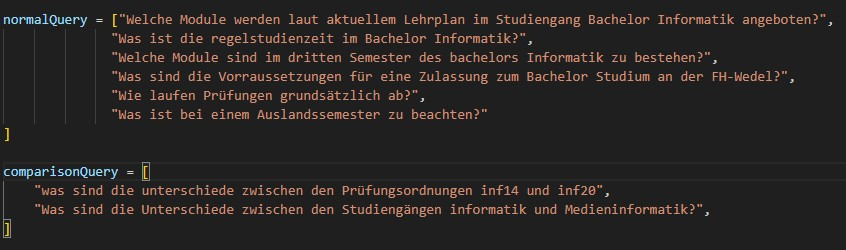
\includegraphics[width=1.0\textwidth]{bilder/queries}\\
    \caption{End-To-End Evaluation}
    \label{fig:e2e}
\end{figure}

\section{Ergebnisse}
Die Metriken liefern jeweils Punkte von 0 bis 1, wobei die Qualität in 0.25 Schritten gemessen wird. DeepEval erlaubt das include-reason Flag zu setzen und somit die Gründe für die Bewertung mit auszugeben was so aussehen kann:

AssertionError: Metrics: Answer Relevancy (score: 0.0, threshold: 0.5, 
reason: The response completely fails to address the question about 
the ECTS credits for the module Digitaltechnik...)

Während der Tests fielen einige Muster auf, die auf verschiedene Probleme hinwiesen, welche in der Folge direkt behoben werden konnten.

\begin{table}[htbp]
\centering
\begin{tabular}{|l|l|l|}
\hline
\textbf{Muster} & \textbf{Wahrscheinliche Ursache} & \textbf{Lösung} \\
\hline
Answer Relevancy = 0 & LLM liefert keine Antwort & Retrieval verbessern \\
Faithfulness = 0 & LLM halluziniert & Prompt anpassen \\
Contextual Relevancy = 0 & Retrieval Probleme & Parser/Metadaten korrigieren \\
Alle Metriken niedrig & Leeres Retrieval & Qdrant Daten überprüfen \\
\hline
\end{tabular}
\caption{Fehlermuster und Gegenmaßnahmen}
\end{table}


Allgemein geben die Tests Aufschluss darauf was gut funktioniert und wo noch Verbesserungspotential besteht. Fragen zu Prüfungsordnungen bzw.  zu allen PVO, ZLO und SPO ergeben in den meisten Fällen gute Ergebnisse und werden gut bewertet. Auch Modulspezifische Fragen werden korrekt beantwortet, indem das gesuchte Modul und der Studiengang herausgefunden werden und die korrekten Chunks abgerufen werden. Fragen zu Modulübersichten, Faktenfragen, Zulassungsfragen, Prüfungsfragen und Fragen zu allgemeinen Regelungen beantwortet der Chatbot mit einer sehr hohen Erfolgsrate. Besonders die MEtriken AnswerRelevancy und Faithfulness werden in den meisten Fällen bestanden. und auch die Antwortzeiten sind vielversprechend.

Verbesserungspotential besteht bei Vergleichen zwischen Modulen, sowie versionsspezifische Fragen. Hier müssten die Parser noch verfeinert werden, um die genauen Versionen und Dokumenttypen herauszufinden, aber im allgemeinen sind die generierten Antworten des Chatbots gut und für sehr spezifische Fragen können in der Zukunft eigene Tools in den Prozess integriert werden, um die Genauigkeit zu verbessern. Die Metrik bezüglich der Kontextuellen Relevanz der abgerufenen Chunks schlägt noch relativ häufig fehl, da zu viele irrelevante Chunks in den TOP-K Chunks sind, allerdings ist der Threshhol dieser Metrik auch nur 0.25 und könnte angepasst werden. Die generierten Antworten sind hierbei oft korrekt, allerdings sorgt der hohe Kontextuelle \enquote{Lärm} für ein Fehlschlagen der Tests.



\chapter{Guardrails mit \emph{NeMo}}
\chapter{Design und Entwicklung des Frontends}

\chapter{MCP Server Entwicklung und Integration}
\chapter{Wie wird das Projekt gestartet?}
\label{chap: anleitung}

Der einfachste Weg, das Projekt vollständig zum Laufen zu bringen, führt über
\emph{Docker} und \emph{Docker Compose}. Alle benötigten Dienste -- Frontend,
RAG-API, Vektordatenbank und Chat-Persistenz -- sind in einer einzigen
\texttt{docker-compose.yml} beschrieben und lassen sich mit wenigen Befehlen starten.

\section{Voraussetzungen}

Folgende Software muss auf dem Zielsystem installiert sein:

\begin{itemize}
    \item \textbf{Docker} (inkl. Docker Compose v2)
    \item Ein \textbf{OpenAI-kompatibler API-Zugang} -- entweder ein echter OpenAI API Key
    oder ein lokal laufendes Modell, das die OpenAI-API emuliert
    (z.\,B. \emph{Ollama} oder \emph{LM Studio})
\end{itemize}

\section{Konfiguration}

Vor dem ersten Start muss die Umgebungskonfiguration eingerichtet werden.
Dazu wird die mitgelieferte Beispieldatei kopiert:

\begin{lstlisting}[language=bash, caption={Konfigurationsdatei anlegen}]
cp .env.example .env
\end{lstlisting}

In der \texttt{.env}-Datei wird festgelegt, welcher LLM-Dienst verwendet werden soll.
Je nach Szenario sind unterschiedliche Einträge relevant:

\begin{itemize}
    \item \textbf{OpenAI API}: \texttt{OPENAI\_API\_KEY} auf den eigenen Key setzen,
    \texttt{OPENAI\_BASE\_URL} auf \texttt{https://api.openai.com/v1}.
    \item \textbf{Ollama (lokal)}: \texttt{OPENAI\_API\_KEY=dummy},
    \texttt{OPENAI\_BASE\_URL=http://url/}.
    \item \textbf{LM Studio}: \texttt{OPENAI\_BASE\_URL=http://host.docker.internal:1234/v1}.
\end{itemize}

\section{Erster Start: Daten laden und indizieren}

Beim allerersten Start müssen die Dokumente der FH Wedel heruntergeladen
und in die Vektordatenbank eingespeist werden. Dazu stehen zwei auskommentierte
Setup-Dienste in der \texttt{docker-compose.yml} bereit, die bei Bedarf aktiviert
werden können. Alternativ lassen sich die Skripte auch direkt ausführen:

\begin{lstlisting}[language=bash, caption={Dokumente herunterladen und indizieren}]
# PDFs von der FH-Wedel-Website herunterladen
python rag-code/download_pdfs.py

# Dokumente verarbeiten und in Qdrant einbetten
python rag-code/indexing_pipeline.py
\end{lstlisting}

Der Indizierungsschritt kann je nach Anzahl der Dokumente und verwendetem Modell
einige Minuten bis zu einer halben Stunde in Anspruch nehmen, da für jedes
Dokument Embeddings berechnet und in \emph{Qdrant} gespeichert werden.
Dieser Schritt muss nur einmalig durchgeführt werden -- die Daten bleiben
in einem Docker-Volume erhalten.

\section{Starten der Anwendung}

Sind die Dokumente indiziert, genügt ein einzelner Befehl, um alle Dienste
hochzufahren:

\begin{lstlisting}[language=bash, caption={Alle Dienste starten}]
docker compose up frontend -d
\end{lstlisting}

Durch die Abhängigkeitsstruktur in der \texttt{docker-compose.yml} werden dabei
automatisch auch alle anderen benötigten Dienste gestartet. Nach kurzer Initialisierungszeit
sind die Dienste über folgende Adressen erreichbar:

\begin{itemize}
    \item \textbf{Frontend} (Next.js-Weboberfläche): \texttt{http://localhost:3000}
    \item \textbf{RAG-API} (FastAPI-Backend): \texttt{http://localhost:8000}
    \item \textbf{Qdrant-Dashboard}: \texttt{http://localhost:6333/dashboard}
    \item \textbf{MongoDB}: \texttt{localhost:27017}
\end{itemize}

Die Weboberfläche unter Port 3000 ist der primäre Einstiegspunkt für den Endnutzer.
Dort kann nach der Auswahl eines Studiengangs direkt mit dem Chatbot interagiert werden.

\section{Nutzung der CLI-Schnittstelle}

Alternativ zur Weboberfläche steht eine interaktive Kommandozeilenschnittstelle
zur Verfügung. Diese ist besonders während der Entwicklung oder für schnelle
Tests praktisch:

\begin{lstlisting}[language=bash, caption={CLI-Modus starten}]
docker compose run --rm rag-cli
\end{lstlisting}

\section{Logs und Fehlerdiagnose}

Die Logs aller laufenden Dienste lassen sich mit folgendem Befehl verfolgen:

\begin{lstlisting}[language=bash, caption={Logs beobachten}]
docker compose logs -f
\end{lstlisting}

Zum Stoppen aller Dienste:

\begin{lstlisting}[language=bash, caption={Alle Dienste stoppen}]
docker compose down
\end{lstlisting}

\section{Hinweise zur Entwicklung}

Für die aktive Entwicklung am Projekt sind in der \texttt{docker-compose.yml}
Bind-Mounts eingerichtet, sodass Änderungen am Quellcode im laufenden Container
direkt sichtbar sind. Das Backend startet mit dem Flag \texttt{--reload}, was
bei Dateiänderungen einen automatischen Neustart des \emph{uvicorn}-Servers
auslöst. Gleiches gilt für das Next.js-Frontend, das im Entwicklungsmodus
ebenfalls mit Hot Reload betrieben wird.

\chapter{Fazit}

... und hier der Schluss.
\end{onehalfspace}

%%%%%%%%%%%%%%%%%%%%%%%%%%%%%%%%%%%%%%%%%%%%%%%%%%%%%%%%%%%%%%%%%%%

\pagenumbering{Roman}
\setcounter{page}{4}

\printbibliography{} % create with BibTeX, gives "chapter without number" warning in log

\appendix
\include{stuff/anhang}

\end{document}
